\documentclass{article}
\usepackage[utf8]{inputenc}
\usepackage[top=1in, bottom=1in, left=1in, right=1in]{geometry}

\usepackage{indentfirst}

\usepackage{url}

\usepackage{biblatex}
\addbibresource{A3_Henriod.bib}

\usepackage{graphicx}
    \DeclareGraphicsExtensions{.png, .jpeg}
\usepackage{wrapfig}
% \usepackage{caption}

\usepackage{amssymb}

%%%

\title{CS791m: A3}
\author{Terence Henriod}
\date{\today}

\begin{document}

\clearpage            % All of
\maketitle            % this,
\thispagestyle{empty} % removes the page number from the title page

\begin{abstract}
A survey of \emph{Ambient Interfaces} (AmIs) - interfaces with \emph{Ambient Intelligence} systems. The past, present, and probable future of AmIs are discussed; the relevance of the subject to the author is also discussed. Related Topics: Ubiquitous Computing, Internet of Things (IoT), Context-aware Computing
\end{abstract}

\newpage
\section{Introduction}
The world of computing is entering a new age, an age where computers are everywhere. Not the everywhere of the 1980s and 1990s with the advent of the personal computer; not the everywhere of the 2000s with personal computers, tablets, and smart phones; but rather an everywhere where many of the devices around us have computers embedded in devices all around us.

Unlike the everywheres of old, humans will not interface with these new computers in the dedicated manner they once did - there will simply be too many computers and devices. Instead, these computers will need to gather their input from human users (for the most part) surreptitiously, and display their information in ways that are commensurate to the ways those devices collected their information. Interfaces that exist in the periphery of our lives are known as \emph{ambient interfaces}.
 \begin{wrapfigure}{R}{0.5\textwidth}
  \begin{center}
    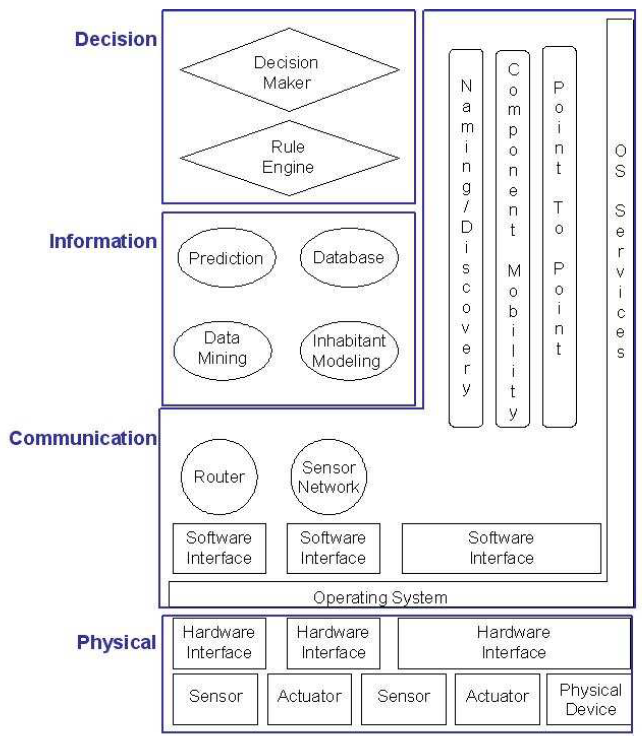
\includegraphics[width=.8\linewidth]{ami_arch}
  \end{center}
  \caption{The typical architecture of a "smart environment". Systems with that seek to create an ambient interface will have strong development in the physical and information components. \cite{Cook:2007:SOE:1225943.1226005}}
  \label{ami_arch}
\end{wrapfigure}

Ambient interfaces will accept their inputs from sensors or by processing data streams generated by our activities; not from direct manipulation by a user. Ambient displays will seek to use spaces and media that currently remain largely unintegrated.
 
The topic of ambient interfaces is actually a subset of \emph{ambient intelligence}, but as the focus here is human-computer interaction, we narrow to the topic of \emph{ambient interfaces}. Both will be abbreviated as AmI. Other associated (or even synonomous) topics include Internet of Things (IoT) and Ubiquitous or Pervasive Computing, and Context-aware Computing. According to Sadri: "The AmI vision may be thought of as the convergence of at least three areas of computing: ubiquitous computing, sensor network technology, and artificial intelligence." \cite{Sadri:2011:AIS:1978802.1978815} All of these topics connote a world where computing devices are interwoven with artifacts of daily life and fade into the background \cite{Cook2009277}.

\begin{table}[h]
  \centering
  \begin{tabular}{| p{5cm} | c | c | c | c | c | c |}
  \hline
  Definition & Sensitive  & Responsive & Adaptive   & Transparent & Ubiquitous & Intelligent \\
  \hline\hline
  A developing technology that will increasingly make our everyday environment sensitive and responsive to our presence
             & \checkmark & \checkmark &            &             &            &             \\
  \hline
  A potential future in which we will be surrounded by intelligent objects and in which the environment will recognize the presence of persons and will respond to it in an undetectable manner
             & \checkmark & \checkmark &            & \checkmark  & \checkmark &             \\
  \hline
  "Ambient Intelligence" implies intelligence that is all around us
             &            &            &            &             & \checkmark & \checkmark  \\
  \hline
  The presence of a digital environment that is sensitive, adaptive, and responsive to the presence of people
             & \checkmark & \checkmark & \checkmark &             &            &             \\
  \hline
  A vision of future daily life . . . contains the assumption that intelligent technology should disappear into our environment to bring humans an easy and entertaining life
             &            & \checkmark &            & \checkmark  & \checkmark &             \\
  \hline
  A new research area for distributed, non-intrusive, and intelligent software systems
             &            &            &            & \checkmark  &            & \checkmark  \\
  \hline
  In an AmI environment people are surrounded with networks of embedded intelligent devices that can sense their state, anticipate, and perhaps adapt to their needs
             & \checkmark &            & \checkmark & \checkmark  & \checkmark & \checkmark  \\
  \hline
  A digital environment that supports people in their daily lives in a nonintrusive way
             &            &            &            & \checkmark  & \checkmark &             \\
  \hline
  \end{tabular}
  \caption{Features of Ambient Intelligence captured by AmI definitions. Adapted from \cite{Cook2009277}.}
  \label{tab:amifeatures}
\end{table}

%
%
\section{History of Ambient Interfaces}
AmI and associated interfaces are in their nascency. To understand the history of AmI, we must understand the history of computing, at least in a general sense.

\begin{wrapfigure}{R}{0.6\textwidth}
  \begin{center}
    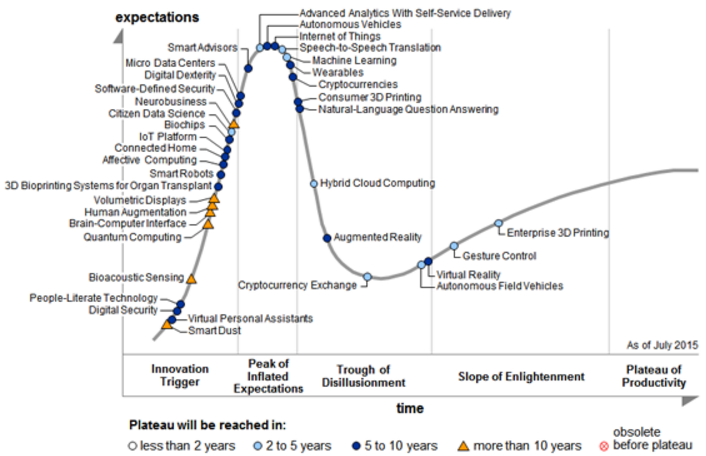
\includegraphics[width=.8\linewidth]{hype}
  \end{center}
  \caption{Gartner's Hype Cycle estimates for 2015. This curve estimates where various technologies are in relation to the potential of their development for society. Note that many of the AmI related technologies are still in the innovation and inflated expectations stages, indicating the newness of the field. \cite{gartner}}
  \label{hype}
\end{wrapfigure}

Early in the history of electronic computers, they were large, complicated machines who only a privileged few has access to. Later, computers became powerful and usable enough that a few more people were able to access them through remote terminals. Then came the personal computer, and it became common for individuals to have a computer in the workplace, home, or both. After that, the progression came to a time when many people carried multiple computing devices on their person, often having some combination of a laptop, tablet, and smart phone.\cite{Cook2009277}

Finally, we come to the age of ubiquitous computing. Computing technology, and its supporting technologies, have reached a point where computers can be embedded anywhere. Lower costs of devices, commoditization of computing, and more have made it easier than ever to add new devices to our lives, and embed computers in devices that may not previously have had or needed computing power. In ubiquitous computing, devices are able to communicate with one another, adding value to a user through cooperation and synergy. These devices can now act on their own and operate remotely or in new places. And of course, these devices can now act with a basic level of intelligence and recognize context (to an extent), allowing them to tailor their actions to situations without user intervention.

AmI research could could not truly be realized until many of the miniaturized, low-cost, and sensor-network technologies became available and stable, only some of the more modest visions for AmI have been realized. That being said, research involving prototype smart homes, wearable electronics, and device-to-device communications have been explored, laying the groundwork. While AmI technology largely remains in the research stages at this point, some estimates foresee (early stage) AmIs making their way into everyday life shortly after 2020 \cite{Sadri:2011:AIS:1978802.1978815}.

%
%
\section{Important Achievements in Ambient Interfaces}
Something \cite{Cook2009277}

%
\subsection{Advent of Ubiquitous Computing}
Much the same way that the automobile industry owes to the major achievements of chemistry, physics, and engineering that made the combustion engine a reality, so too do ambient interfaces owe to the technologies that make ubiquitous computing possible.

No discussion of the advancement computing technology would be complete without referencing Moore's Law. Moore's Law. Moore's Law states that "the integration density of systems on silicon doubles every eighteen months" \cite{Aarts:2009:NRP:1735821.1735822}. Although no longer true, this means that for the last few decades, the amount of technology that could be placed on a chip has increased dramatically, allowing for relatively small packages of sensors, computation hardware, and communication chips\cite{Aarts:2009:NRP:1735821.1735822}. Without a small form factor, AmI technology would not be very "ambient".

Low-power electronics, new battery technologies, and energy harvesting technologies enable the deployment of devices where a standard electrical grid might not be available \cite{5475111}. This allows sensors to be placed in areas without existing infrastructure, be it in an undeveloped area, or simply in a part of a building where there is not an available power outlet. These energy mitigating techniques also lower the barrier to deployment because they reduce concerns around energy consumption.

Without advances in wireless network protocols and messaging frameworks, small devices could not be connected and cooperative. The development of sensor- and sensor-actuator networks has made ubiquitous computing, and therefore AmI, possible. Some of the major protocols and frameworks include ZigBee, Z-Wave, LoRa, AllJoyn, and MQTT. Many more are being developed to help realize true interoperability between devices \cite{elevenprotocols}.


%
\subsection{Functional Smart Home Prototypes}
Several functioning smart home, office, and city environments have been created for the purpose of AmI research and prototype testing \cite{Cook:2007:SOE:1225943.1226005}. These test environments are a major step in taking AmI technologies from the conceptual stage to the later stages of research. These test environments have helped researchers identify many of the issues that AmI technologies might face once they are deployed for real-world use. 

The Aware Home Research Initiative (AHRI), at Georgia Institute of Technology, has created several of these test environments. They have produced the Aware Home, a somewhat large, real house that is outfitted with many research prototypes and infrastructure, where study participants might spend 1-10 days for AmI studies; the AHRI has also created the HomeLab program to test their research under actual living conditions with volunteering seniors, whose homes are outfitted with with products for evaluation. \cite{ahri}

\begin{table}[h]
  \centering
  \begin{tabular}{| c | c | p{7cm} |}
  \hline
  Properties     & Measurand                                          & Example Use Cases \\
  \hline\hline
  Physical       & pressure, temperature, humidity, flow              & climate control, resource usage \\
  \hline
  Motion         & position, velocity, angular velocity, acceleration & detect and predict where a user is going, log physical activity \\
  \hline
  Contact        & strain, force, torque, slip, vibration             & detect when object is in use, provide assistance if necessary \\
  \hline
  Presence       & tactile/contact, proximity, distance/range, motion & room occupancy detection \\
  \hline
  Biochemical    & biochemical agents                                 & safety (hazardous material detection), context recognition (cooking for example)\\
  \hline
  Identification & personal features, personal ID                     & personalization of information, security\\
  \hline
  \end{tabular}
  \caption{Sensors and their uses for smart environments. Adapted from \cite{Cook:2007:SOE:1225943.1226005} and augmented.}
  \label{tab:amisensors}
\end{table}


%
\subsection{Cultural Acceptance of Mobile and Wearable Technology}
A major step in the development of AmI is fostering comfort and acceptance by users. For AmI in particular, this means making users so comfortable with something that they are prepared to interact with technology continuously. The advent and adoption of mobile and wearable technologies signifies this comfort and acceptance.

The smart phone is the epitome of mobile computing technology. Users carry these devices with them everywhere and use them for many of their daily activities. While the main uses of mobile phones require direct interactions on the user's part, these phones often carry many sensors for directly sensing the user or their environment (location, temperature, etc.) or applications that can provide the raw data for AmI purposes (social applications). Mobile devices can be used for ambient displays as well, since they feature screens that are not always in direct use \cite{Cook2009277} \cite{Cook:2007:SOE:1225943.1226005} \cite{Sadri:2011:AIS:1978802.1978815}.

Wearable technologies allow for the most pervasive and least intrusive of interfaces to become a reality (short of devices that might be actually embedded into a person's body, something people may not be comfortable with for some time). Fitness trackers are a prime example of wearable technology that can act as the input side of an AmI \cite{Cook2009277}.

%
%
\section{Current Research and Developments}

%
\subsection{Context Recognition}

\begin{wrapfigure}{R}{0.5\textwidth}
  \begin{center}
    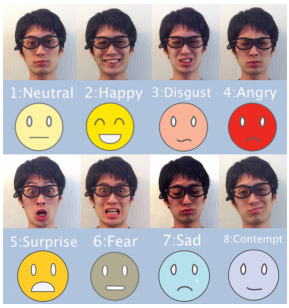
\includegraphics[width=.8\linewidth]{emotion_eyewear}
  \end{center}
  \caption{Prototype eyewhere for recognizing the wearer's emotions. \cite{7390646}}
  \label{emotion-eyewear}
\end{wrapfigure}

Perhaps one of the greatest difficulties for AmI applications will be to develop robust, generalizable context recognition. The idea behind context recognition is to take utilize data to determine what the is currently happening in an environment. Once a context can be determined, an AmI system can take appropriate action for the user's benefit. \cite{Cook2009277} In order to produce robust context recognition, advances in artificial intelligence and machine learning are required, along with techniques to utilize noisy and intermittent sensor data \cite{Sadri:2011:AIS:1978802.1978815} (related: \emph{Opportunistic Context Recognition}). This area is possibly the most important step in producing true AmIs, since it is relatively easier to make unobtrusive sensor environments than it is to produce effective systems that don't need to be directed by a user.

As an example of recent context recognition research, Masai et al produced a prototype of software and sensors embedded into typical eye wear that could detect a wearer's current emotion with moderate success \cite{Masai:2016:FER:2856767.2856770}. Interfaces like these could be used to actuate events conducive to the user's mood without explicit user direction, such as playing appropriate music or notifying others of the mood through social media.

Other efforts have been undertaken to estimate user contexts by combining many different types of data that can be gathered by a mobile phone, and then applying machine learning techniques \cite{Huai:2014:TPC:2672614.2629504}. Using "semi-supervised" learning methods, Huai et al were able to produce models that could estimate user context, albeit at a high level (is the user eating, driving, etc.), effectively.

%
\subsection{Natural Interfaces}
In order to make AmIs actually ambient, interfaces should accept actions users would naturally perform as input. This can include recognizing facial expressions (as described earlier in \cite{Huai:2014:TPC:2672614.2629504}), gesture recognition, or speech recognition  \cite{Cook2009277}. Ideally, a natural interface should not require a user to learn any new skills, only that their existing skills for interacting with other humans are sufficient for interacting with a device or system. Of course, not all natural interfaces are necessarily about direct human-like communication from a user, sometimes, natural interfaces might simply monitor a user's activities as they would normally be performed, perhaps by instrumenting the fixtures of a room or work setting \cite{Baharin:2015:SSI:2798442.2754165}.

\begin{wrapfigure}{R}{0.5\textwidth}
  \begin{center}
    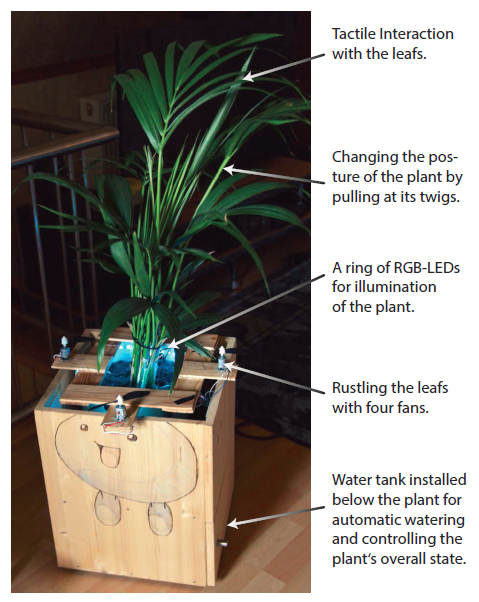
\includegraphics[width=.8\linewidth]{infoplant}
  \end{center}
  \caption{A prototype ambient interface (display) using a natural plant \cite{7390646}}
  \label{infoplant}
\end{wrapfigure}

However, natural interfaces are not entirely about accepting input from a user either. Natural displays might use augmented artifacts and architectures already present such as plants \cite{7390646} or wallpapers \cite{Huang:2005:IW:1086057.1086142}. Such displays can be weaved into our surroundings, presenting information continuously, but only if we wish to attend to them, similar to our current existing surroundings.

%
\subsection{Building Management}
As ecological and financial concerns rise, the desire to efficiently control building environments increases. Businesses and individuals have a vested interest in controlling indoor climates, and AmI can provide the means to do so without human involvement, but with better-than-human performance. Often, approaches to improve the energy efficiency of a building fall into four categories: increasing consumption awareness, reducing standby consumption, activity scheduling, and adaptive control \cite{DePaola:2014:IMS:2620784.2611779}. All are directly relevant to AmI, since all of these can presumably be automated given some user preference profiles and timely data on those users.

While the goals of AmI might be to reduce or even eliminate the need for active human interaction with building systems, unobtrusively displaying information to a user is a goal for AmI systems. Increasing consumption awareness would require such a display; users should be aware if their behavior requires too many resources and should be able to get feedback on their behavior, but in most scenarios this is not the kind of information that merits interruption of other tasks. Attempts have been made to implement such "eco-feedback displays" with encouraging results \cite{7390646}, although "the sole provision of
feedback is not sufficient to ensure significant energy savings in the long term" \cite{DePaola:2014:IMS:2620784.2611779}.

\begin{wrapfigure}{R}{0.5\textwidth}
  \begin{center}
    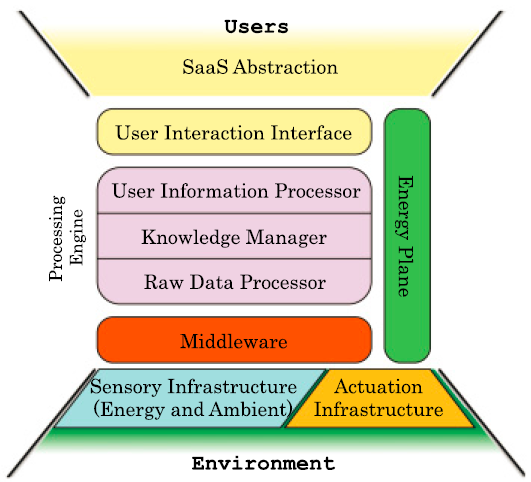
\includegraphics[width=.8\linewidth]{smart_building_architecture}
  \end{center}
  \caption{Architecture of a building management System for energy efficiency. A truly ambeint interface will maximize the autonomy of the sensory and actuation infrastructure. \cite{DePaola:2014:IMS:2620784.2611779}}
  \label{smart-building}
\end{wrapfigure}

Activity scheduling has less to do with the interfaces of AmI, and more to do with the intelligence side (we mention it here for completeness). Activity scheduling involves scheduling certain tasks for times where the most benefit can be achieved; running high energy consumption appliances during the day when electricity prices are low would be an example. Currently, automated systems for such tasks are not in wide use; the more common approach is to help the user determine such schedules by providing easy to use traditional interfaces and attempting to learn such schedules from the user's input. One such example might be the Nest smart home thermostat \cite{nest}, which attempts to learn a user's home occupation patterns in order to tune climate control to save energy.

Reducing standby consumption refers to managing when appliances are left on in standby-mode, or simply shutdown. Appliances in standby-mode might use energy at a lower rate, it is estimated that consumer and office appliances use more energy in standby mode than when in use due to the large amount of time spent in standby mode \cite{DePaola:2014:IMS:2620784.2611779}. AmI could produce an energy savings by powering devices down at appropriate times such as when a room is not occupied or users are engaged in other activities, rather than leaving them in standby mode for extended periods of time.

Adaptive control is likely the area with the most potential for improvement by AmI. Adaptive control involves using context recognition techniques such as presence detection to detect when a system such as an HVAC system or lighting system should be active \cite{DePaola:2014:IMS:2620784.2611779}. It is easy to envision a scenario where an AmI system could utilize data on user presence, physiological state, and outdoor weather conditions to tune the temperature control or to comfortable levels for a user, or adjust lighting levels based on their current activities.

%
\subsection{Rules Engines}
Unfortunately, until truly "intelligent" (as in human-like intelligence) systems can be developed, users do need to program or configure AmI systems to perform correct actions under correct inputs. Researchers hope to progress to developing intelligent agents with "butler-like" capabilities and human-like social skills, but these are incredibly difficult tasks (after all - it can take humans decades to perfect such skills) \cite{Cook2009277} \cite{Cook:2007:SOE:1225943.1226005}. In the mean time, there are many efforts to design convenient rules engines that inter-operate well with many devices.

One such rules engine is If This Then That (IFTTT). IFTTT is a rules engine designed to integrate an AmI with a user's mobile app activities. The user can use IFTTT "recipes" that can automate activities for the user, such as purchasing online media content when a user "likes" something, adding events to a calendar, or logging information for later viewing by the user. Once the user sets up the automation, the rest happens "in the background", without the user's intervention. \cite{ifttt}

\begin{wrapfigure}{R}{0.5\textwidth}
  \begin{center}
    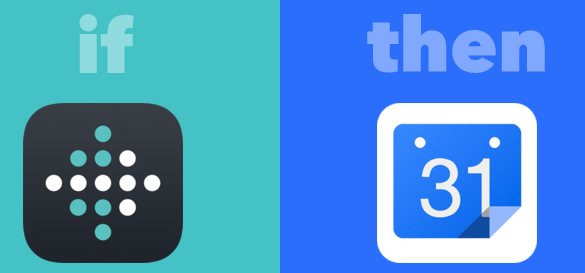
\includegraphics[width=.6\linewidth]{ifttt_recipe}
  \end{center}
  \caption{An example of an IFTTT "recipe". This recipe indicates that if a user's FitBit (a fitness tracking wearable) detects that the user did not get sufficient sleep the previous night, then IFTTT will automatically create a reminder for the user in their (Google) Calendar app to go to sleep on time. \cite{ifttt}}
  \label{ifttt_recipe}
\end{wrapfigure}

An example of a more industrial strength rules engine is the Amazon Web Services IoT platform. The AWS IoT platform is an industrial strength cloud platform designed to integrate many, arbitrary devices together, processing the information they send and sending messages to other devices based on rules designed around incoming messages. \cite{awsiot}


\subsection{Enhanced Socialization}
A major concern with the increased computerization of our world is that it will increase the remoteness of individuals from one another, driving us towards a society of introverts. For this reason, work is being done to help the increased computerization of our society better connect us with each other.

AmI has the potential to increase human-human interactions through information sharing. By ambiently or directly gathering data from users, AmIs can then display that information to other users when relevant, fostering interaction. Sharing of user-profiles, displaying status, or alerting others if need arises are all vehicles for this kind of facilitation \cite{Sadri:2011:AIS:1978802.1978815}.

The SonicAIR project aimed to foster a sense of connection between individuals living at different locations by recording user kitchen activities through several sensors, and then representing those activities to the other users using sound icons. Users reported feeling more aware of those in the other locations, and feeling more connected through learning some of their habits \cite{Baharin:2015:SSI:2798442.2754165}.

%
%
\section{Major Players}

%
\subsection{Georgia Tech (Academia)}
Georgia Tech is certainly a major player in the AmI space given that it is home to both the previously mentioned AHRI \cite{ahri} and the Ubicomp Group \cite{gtubicomp} (likely a more modern iteration of AHRI). The Georgia Tech Ubicomp Group conducts research an many areas applicable to ubiquitous computing (and therefore synonymously ambient interfaces). They have been publishing research since 2011, so their work is fairly new, but still distinctive. Their research focuses include: "automated capture and access to live experiences, context-aware computing, applications and services in the home, natural interaction for mobile and wearable computing, software architecture, security and privacy issues, technology for individuals with special needs, and personal informatics" \cite{gtubicomp} - all things directly related to AmI.

%
\subsection{Philips (Industry)}
Philips is a technology company invested in creating new, life changing innovations. Philips is a major player in IoT innovations, and many of their products are medical and health-care oriented. According to some, Philips was the one that actually coined the term "ambient intelligence" in the 1990s. Acting in both the consumer and industrial markets, Philips has been, and is likely to continue to be, a leader in ambient interfaces. \cite{philips}


%
\subsection{Human-Computer Interaction Institute of Carnegie Mellon}
\begin{wrapfigure}{R}{0.3\textwidth}
  \begin{center}
    
\includegraphics[width=.6\linewidth]{hcii}
  \end{center}
  \caption{Human Computer Interaction Institute of Carnegie Mellon logo. \cite{hciicmu}}
  \label{hcii}
\end{wrapfigure}
Carnegie Mellon University is a well known, top-tier institution in general, but it is certainly well established in terms of HCI. They are also well established in what they refer to as "context-aware computing". In terms of volume of research, they are the most prolific institution for publications when searching the ACM digital library for "ambient intelligence". The HCII at CMU has a variety of ambient interface work in progress including emotion recognition from audio, human routine modeling, and characterization of the personal relationships people have with technology. \cite{hciicmu}

%
%
\section{Expected Research and Developments}

%
\subsection{Security and Privacy}
According to many sources, protocols and security measures need to be well defined for AmI technologies \cite{Cook2009277} \cite{Sadri:2011:AIS:1978802.1978815}. This is obviously true in the sense that many interconnected devices have the possibility to become a bot-net, but also in the sense that AmI will produce large amounts of personal data. Since the focus of this survey is not computer security, we would like to make it clear that we are referring to the security and privacy of how user's data is collected by an interface and how it is used or displayed.

AmIs should work to collect users data discreetly and without causing the user to have to change their behavior in any way. While this is not always possible, since user's might change their behavior simply by virtue that it is being observed, it should be done in a way that does not require the user to hide the behavior observed by ambient interfaces. Also, on the other side of an interface, the display, should the display be public in any way, researchers will likely need to engineer ways to share the data without getting too personal (as was done in \cite{Baharin:2015:SSI:2798442.2754165}).

%
\subsection{Mobile and Wearable Technologies}
We expect AmI research using mobile phones and wearable devices to continue well into the future. Their adoption by society and their capabilities to collect data directly from a user wherever the user goes makes these technologies prime candidates for ambient interface research.

Already, research is being done with these technologies for purposes of health monitoring, location/context finding, context, and (sometimes) unobtrusive notifications of events. It is very likely that this trend will continue, particularly in the areas of context and and health monitoring. Using ambient interfaces to track the status of a user has high potential in terms of disease prevention or emergency notifications - high priorities in research areas such as independent living for seniors \cite{Cook2009277} \cite{Sadri:2011:AIS:1978802.1978815}. 

%
\subsection{Natural and Unobtrusive Displays}
Since ambient interfaces seek to display information to a user in a non-intrusive and artful way, for the most part, continued research in more fully utilizing existing artifacts and architecture is likely. Examples of displays that fill non-traditional (non-screen) spaces include plants, walls, statues, sounds, etc. While research of this nature is currently occurring, it is likely that it will continue in order to determine what modalities are effective in information display as well as cost.

Soundscapes are a likely candidate for continued research in ambient displays. Audio is a relatively unexploited outside of traditional interfaces (that tend to have screens), but practical medium for relaying information in an ambient manner. Certainly movies and video-games use audio in this way already, and to some extent, other direct interfaces (like in vehicles), so it is feasible that audio could be used in other, less virtual, environments as well \cite{Baharin:2015:SSI:2798442.2754165}.

Of course, existing artifacts can be modified or created also. There has been a lot of research in this area using natural and robotic plants \cite{7390646}, shape-shifting desk statues \cite{Jafarinaimi:2005:BAD:1056808.1057063}, and wall-papers \cite{Huang:2005:IW:1086057.1086142}. This research appears to be continuing in a strong way, and given that there are a great many artifacts around us that remain unused, this type of research is likely to continue. Further, the true effectiveness of these displays remains to be seen, as many of the studies in these areas have few participants.

%
%
\section{Contribution to My Studies}
The area of Internet of Things, and more specifically, ambient interfaces, contributes to my studies in two ways.

First, it is an area that I find interesting. this provides motivation and content for my efforts in class projects. I find this areas to be interesting because, like many others, I think this is the next step in computing evolution for humanity. I think that the applications and implications are numerous, ans that this is the next (and possibly largest, thus far) step in creating the automated, Utopian kind of world that we often dream of in science fiction and movies.

Second, my current employment is with a company that focuses on a related area (if it is any different than this). So studying the topics of this area are conducive to my professional development if I continue to remain working in this space.

%
%
\section{Conclusion}
In this paper we have explored the current state of the field of \emph{ambient interfaces}. Ambient interfaces seek to both enhance and eliminate direct human interaction with computers by unobtrusively collecting data and displaying output. Current and future research in the space was discussed, as well as major players in the field.

%
%
\printbibliography

%
\end{document}